\section{Preliminaries}
\subsection{Event Structure \cite{es}}
\begin{definition}[Event Structure]
    An event structure is a triple $\mr{E} = (E,\#,\vdash)$ where:
    \begin{enumerate}
        \item $E$ is a set of events
        \item \# is a binary symmetric, irreflexive relation on $E$,
              the conflict relation.
              We shall write $Con$ for the set of conflict-free subsets of $E$,
              i.e. those finite subsets $X \subseteq E$ for which:
              $\forall e,e' \in X . \neg (e\#e')$
        \item $\vdash \subseteq Con \times E$ is the enabling relation which satisfies:
              $ X \vdash e \ \& \ X \subseteq Y \in Con \Rightarrow Y \vdash e$
    \end{enumerate}

\end{definition}
\begin{notion}
    In an event structure we shall write $\doublevee$ for the reflexive conflict relation by which we mean
    that $e\doublevee e'$ in an event structure iff either $e\#e'$ or $e=e'$.
    With this notion instead of describing the conflict-free sets of an event structure
    as those sets $X$ such that
    \begin{align*}
        \forall e,e' \in X. \neg(e\#e')
    \end{align*}
    we can say they are those sets $X$ for which:
    \begin{align*}
        \forall e,e' \in X. e\doublevee e' \Rightarrow e=e'
    \end{align*}
\end{notion}

\begin{notion}
    For any event structure we can define the minimal enabling relation $\vdash_{min}$ by:
    \begin{align*}
        X \vdash_{min} e \iff X \vdash e \wedge
        ( \forall Y \subseteq X . Y \vdash e \Rightarrow Y = X )
    \end{align*}
    Then for any event structure:
    \begin{align*}
        Y \vdash e \Rightarrow \exists X \subseteq Y . X \vdash_{min} e
    \end{align*}
\end{notion}

\begin{definition}[Configuration]
    \label{conf}
    Let $\mr{E} = (E,\#,\vdash)$ be an event structure.
    Define a configuration of $\mr{E}$ to be a subset of events $x \subseteq E$ which is
    \begin{enumerate}
        \item conflict-free: $x \in Con$
        \item secured: $\forall e \in x. \exists e_0,...,e_n \in x. e_n = e \ \wedge
                  \forall i \leq n. \s{e_0,...,e_{i-1}} \vdash e_i$
    \end{enumerate}
\end{definition}
The set of all configurations of an event structure is written as $\mathcal{F}(E)$.
It is helpful to unwrap condition (2) a little. It says an event $e$ is secured in a set $x$
iff there is a sequence of events $e_0,...,e_n = e$ in $x$ such that:
\begin{align*}
    \emptyset \vdash e_0, \s{e_0} \vdash e_1, ..., \s{e_0,...,e_{i-1}} \vdash e_i,...,
    \s{e_0,...,e_{n-1}} \vdash e_n.
\end{align*}
We call such a sequence $e_0,e_1,...,e_n = e$ a \emph{securing} for $e$ in $x$.
We use $X \subseteq_{fin} Y$ to mean $X$ is a finite subset of $Y$.

\begin{example}
    Consider another network in which two hosts are connected
    to a single switch.
    This time both hosts are sending a packet concurrently to the
    host.
    Once the switch received a packet from either host it will
    drop the packets received from the other host due to capacity
    limit.
    \begin{center}
        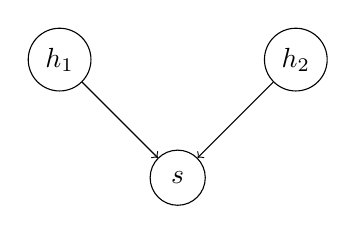
\begin{tikzpicture}[node distance={15mm},minimum width=7mm,main/.style = {draw, circle}]
            \node[main] (S) {$s$};
            \node[main] (H1) [above of=S,left of=S] {$h_1$};
            \node[main] (H2) [above of=S,right of=S] {$h_2$};
            \draw[->] (H1) -- (S);
            \draw[<-] (S) -- (H2);
        \end{tikzpicture}
    \end{center}
    Let $r_1,r_2$ represent the events of receiving packet from
    $h_1$ and $h_2$ and $d_1,d_2$ represent the events of dropping
    packets from these hosts.
    We need a conflict relation the least one for which we have
    $r_1\#d_1$ and $r_2\#d_2$
    and enabling relation the least one that satisfies:
    \begin{align*}
        \emptyset & \vdash_{min} r_1 \\
        \emptyset & \vdash_{min} r_2 \\
        \s{r_1}   & \vdash_{min} d_2 \\
        \s{r_2}   & \vdash_{min} d_1 \\
    \end{align*}
    Thus the configurations have the form:
    \begin{center}
        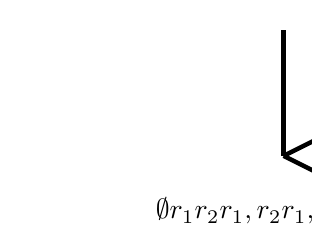
\begin{tikzpicture}[scale=0.8]
            \crd{0}{0}{$\emptyset$}
            \crd[left]{-2}{1}{$\s{r_1}$}
            \crd[right]{2}{1}{$\s{r_2}$}
            \crd[right]{0}{2}{$\s{r_1,r_2}$}
            \crd{-2}{3}{$\s{r_1,d_2}$}
            \crd{2}{3}{$\s{r_2,d_1}$}
            \draw [ultra thick] (0,0) -- (2,1);
            \draw [ultra thick] (0,0) -- (-2,1);
            \draw [ultra thick] (-2,1) -- (0,2);
            \draw [ultra thick] (2,1) -- (0,2);
            \draw [ultra thick] (-2,1) -- (-2,3);
            \draw [ultra thick] (2,1) -- (2,3);
        \end{tikzpicture}
    \end{center}
\end{example}

\subsubsection{Stable Event Structure}

We look for a special class of event structures for which there is a
the partial order of causal dependency on each configuration.
This can not be done so obviously for all event structures.
Consider the event structure of the previous example in which
the event $b$ causally depends not on a unique set of events
but rather on either the occurrence of 0 or on the occurrence of 1.
It is incorrect to say $b$ causally depends on both 0 and 1 because
the occurrence of only one of them enables the occurrence of $b$.
The difficulty arises because there is a configuration $\s{0,1,b}$
in which there is an event $b$ which is not enabled by a unique minimal
set of event occurrences.
We can rule out such possibilities by insisting on event structures
satisfy the following stability axiom.
\begin{definition}[Stable Event Structure]
    Let $\mr{E} = (E,\#,\vdash)$ be an event structure. Say $E$ is stable if it satisfies the following axiom:
    \begin{align*}
        X \vdash e \ \wedge \ Y \vdash e \ \wedge \ X \cup Y \cup \{e\} \in Con \Rightarrow X \cap Y \vdash e
    \end{align*}
\end{definition}
The stability axiom ensures that an event in a configuration is
enabled in an essentially unique way.
Assume $e$ belongs to a configuration $x$ of a stable event structure.
Suppose $X \vdash e$ and $X \subseteq x$.
Then $X \cup \s{e} \in Con$, the enabling $X\vdash e$ is consistent.
Take
\begin{align*}
    X_0 = \bigcap \s{Y ~|~ Y \subseteq X \wedge Y \vdash e}
\end{align*}
Because $X$ is finite this is an intersection of a finite number of
sets and we see by the stability axiom that $X_0 \vdash e$.
Moreover $X_0$ is the unique minimal subset of $X$ which enables $e$.
Thus for stable event structures, we have:
\begin{align*}
    Y \vdash e \wedge Y \cup \s{e} \in Con \Rightarrow
    \exists ! X \subseteq Y.X \vdash_{min} e
\end{align*}
It follows that for stable event structures
\begin{align*}
    X \vdash_{min} e \wedge Y \vdash_{min} \wedge
    X \cup Y \cup e \in Con \Rightarrow X = Y
\end{align*}
\begin{definition}
    Let $\mr{E_0} = (E_0,\#_0,\vdash_0)$ and $\mr{E_1} = (E_1,\#_1,\vdash_1)$
    be event Structures. Define
    \begin{align*}
        \mr{E_0} \trianglelefteq \mr{E_1} \iff
         & E_0 \subseteq E_1,                            \\
         & \forall e,e'. e\#_0e'  \iff e,e' \in E_0
        \ \wedge \ e\#_1 e' \text{ and }                 \\
         & \forall X,e.X\vdash_0 e  \iff X \subseteq E_0
        \ \wedge \ e \in E_0\ \wedge \ X \vdash_1 e
    \end{align*}
    In this case say $\mr{E_0}$ is a substructure of $\mr{E_1}$.
\end{definition}

\begin{definition}[Restriction]
    Let $\mr{E} = (E,\#,\vdash)$ be an event structure.
    Let $A \subseteq E$.
    Define the restriction of $\mr{E}$ to $A$ to be
    \begin{align*}
        \mr{E} \lceil A = (A,\#_A,\vdash_A)
    \end{align*}
    where
    \begin{align*}
        X \in Con_A \iff X \subseteq A \ \wedge \ X \in Con \\
        X \vdash_A e \iff X \subseteq A \ \wedge \ e \in A \ \& \ X \vdash e
    \end{align*}
\end{definition}

\begin{definition}
    Let $a$ be an event.
    For an event structure $\mr{E} = (E,\#,\vdash)$ define $a\mr{E}$ to be the event structure $(E',\#',\vdash')$ where:
    \begin{align*}
         & E' = \s{(0,a)} \cup \s{(1,e)|e \in E},                                                                               \\
         & e_0' \#' e_1'  \iff \exists e_0,e_1.e_0' = (1,e_0)
        \ \wedge \ e_1' = (1,e_1) \ \wedge \ e_0 \# e_1                                                                         \\
         & X \vdash' e' \iff e' = (0,a) \text{ or } [e' = (1,e_1) \ \wedge \ (0,a)\in X \ \wedge \ \s{e|(1,e)\in X} \vdash e_1]
    \end{align*}
\end{definition}

\begin{definition}
    A labelled event structure consists of $(E,\#,\vdash,L,l)$ where
    $(E,\#,\vdash)$ is an event structure, $L$ is a set of labels,
    not including the element *, and $l$ is a function $l: E \rightarrow L$
    from its events to its labels.
\end{definition}
\subsection{Causal Model \cite{hp}}

A signature $\mathcal{S}$ is a tuple $(\mathcal{U},\mathcal{V},\mathcal{R})$,
where $\mathcal{U}$ is a set of exogenous variables, $\mathcal{V}$
is a set of endogenous variables, and $R$ associates with every variable
$Y\in \mathcal{U}\cup \mathcal{V}$ a nonempty set $\mathcal{R}(Y)$ of possible values for $Y$.
A causal model (or structural model) over signature $S$ is a tuple
$M=(\mathcal{S},\mathcal{F})$, where $\mathcal{F}$ associates with
each variable $X \in \mathcal{V}$ a function denoted $F_X$ such that
$F_X: (\times_{U\in \mathcal{U}}\mathcal{R}(U))\times (\times_{Y\in\mathcal{V}-\{X\}}\mathcal{R}(Y))\rightarrow \mathcal{R}(X)$.

$F_X$ determines the value of $X$ given the values of all the other variables
in $\mathcal{U}\cup \mathcal{V}$.
For example, if $F_X(Y,Z,U)=Y+U$ (which we usually write as $X = Y + U$),
then if $Y=3$ and $U=2$, then $X = 5$, regardless of how $Z$ is set.
These equations can be thought of as representing processes (or mechanisms) by which values are assigned to variables. Hence, like physical laws, they support a counterfactual interpretation.
For example, the equation above claims that in the context $U=u$, if $Y$ were 4, then $X$ would be $u+4$ (which we write as $(M,u) \models [Y\leftarrow 4](X = u + 4))$, regardless of what values X, Y, and Z actually take in the real world.


The function $\mathcal{F}$ defines a set of (\textit{modifiable}) \textit{structural equations} relating to the values of the variables.

\begin{example}
    Suppose that we want to reason about a forest fire that could
    be caused by either lightning or a match lit by an arsonist.
    Then the causal model would have the following endogenous variables :
    \begin{itemize}
        \item $F$ for fire
        \item $L$ for lighting
        \item $ML$ for match lit
    \end{itemize}
    The set $\mathcal{U}$ of exogenous variables includes conditions
    that suffice to render all relationships deterministic (such as
    whether the wood is dry, whether there is enough oxygen in the air
    for the match to light, etc.).
    Suppose that $\vec u$ is a setting of the exogenous variables that
    makes a forest fire possible (i.e., the wood is sufficiently dry,
    there is oxygen in the air, and so on).
    Then, for example, $F_F(\vec u, L, ML)$ is such that $F=1$ if either
    $L=1$ or $ML=1$.
    Note that although the value of $F$ depends on the value $L$ and $ML$, the value of $L$ does not depend on the values of $F$ and $ML$.
\end{example}

\subsubsection{Causal Network}
We can describe a causal model $\m$ using a causal network.
This is a graph with nodes corresponding to the random variables
in $\mathcal{V}$ and an edge from a node labeled $X$ to one
labeled $Y$ if $F_Y$ depends on the value of $X$.
This graph is a dag that follows from the assumption that the
equations are recursive.
We occasionally omit the exogenous variables $\vec U$ from the causal network.
For example, the causal network for example 2.2.1 has the following
form:

\begin{center}
    \begin{tikzpicture}[node distance={15mm}]
        \node (l) {L};
        \node (ml) [below right of=l]  {ML};
        \node (f) [above right of=ml] {F};
        \draw [->] (l) -- (ml);
        \draw [->] (f) -- (ml);
    \end{tikzpicture}
\end{center}

\subsubsection{Actual Cause}
Given a signature $S= (\mathcal{U},\mathcal{V},\mathcal{R})$, a formula of the form $X =x$, for $X \in \mathcal{V}$ and $x \in \mathcal{R}(X)$, is called a \textit{primitive event}.
A \textit{basic causal formula} is one of the form $[Y_1 \leftarrow y_, ..., Y_l\leftarrow y_k]\varphi$, where $\varphi$ is a Boolean combination of primitive events, $Y_1,...,Y_k$ are distinct variables in $\mathcal{V}$, and $y_i \in \mathcal{R}(Y_i)$.
Such a formula is abbreviated as $[\vec{Y}\leftarrow\vec{y}]\varphi$.
A \textit{causal formula} is a Boolean combination of basic causal formulas.
A causal formula $\psi$ is true or false in a causal model, given a context.
We write $(M,\vec u)\models \psi$ if $\psi$ is true in causal model $M$ given context $\vec u$.
$(M,\vec u)\models [\vec Y\leftarrow \vec y](X=x)$ if the variable $X$ has value $x$ in the unique solution to the equation in $M_{\vec{Y} \leftarrow \vec{y}}$ in context $\vec u$.
The context and structural equations are given.
They encode the background knowledge.
All relevant events are known.
The only question is picking out which of them are the cause of $\varphi$ or, alternatively, testing whether a given set of events can be considered the cause of $\varphi$.
The types of events that we allow as actual causes are ones of the form $X_1 = x_1 \wedge ... \wedge X_k=x_k$-- that is, conjunctions of primitives events.
We abbreviate this as $\vec X = \vec x$.
\begin{definition}
    $\vec X = \vec x$ is an actual cause of $\varphi$ in $(M,\vec u)$ if the following three conditions hold:
    \begin{itemize}
        \item  \textbf{AC1.} $(M,\vec u)\models (\vec X = \vec x) \wedge \varphi$.
              (both $\vec X = \vec x$ and $\varphi$ are true in actual world)
        \item  \textbf{AC2. }There exists a partition $(\vec Z, \vec W)$ of $\mathcal{V}$ with $\vec X \subseteq \vec Z$ and some setting $(\vec x',\vec w')$ of the variables in $(\vec X,\vec W)$ such that if $(M,\vec u)\models \vec Z = z^*$ for all $Z\in \vec Z$, then both of the following conditions hold:

              (a) $(M,\vec u)\models[\vec X \leftarrow \vec x', \vec W \leftarrow \vec w']\neg \varphi$.

              (b) $(M,\vec u)\models[\vec X\leftarrow \vec x, \vec W' \leftarrow \vec w', \vec Z'\leftarrow \vec z^*]\varphi$ for all subsets $\vec W'$ of $\vec W$ and all subsets $Z'$ of $\vec Z$.

        \item  \textbf{AC3.} $\vec X$ is minimal; no subset of $\vec X$ satisfies conditions $AC1$ and $AC2$.
    \end{itemize}
\end{definition}
We call the tuple $(\vec W, \vec w,\vec x')$ a witness to the fact that $\vec X=\vec x$ is a cause of $\varphi$.

\begin{definition}
    We say $\vec X = \vec x$ is a but-for cause of $\varphi$ in
    $(M,\vec u)$ if there exists a witness $(\vec W, \vec w, \vec x')$
    for $\vec X = \vec x$ being an actual cause of $\varphi$
    where $\vec W = \emptyset $.
\end{definition}

Note that, if we consider a witness $(\vec W, \vec w, \vec x')$
for checking whether $\vec X = \vec x$ is a cause of $\varphi$
in $(M,\vec u)$ where $\vec W = \e$, then in the AC2(b) condition
we only need to check whether $(M,\vec u) \vDash [\vec X \leftarrow \vec x, \vec Z' \leftarrow \vec z^*]\varphi$ for all subsets $\vec Z'$
of $\vec Z$.
Since we have $(M,\vec u) \vDash (\vec X = \vec x)$ and
$(M,\vec u) \vDash Z = z^*$ for all $Z \in \vec Z$,
the Interventions $\vec X \leftarrow \vec x$ and
$\vec Z ' \leftarrow \vec z^*$ actually do not change the value of
any variable thus checking whether
$(M,\vec u) \vDash [\vec X \leftarrow \vec x, \vec Z' \leftarrow \vec z^*]\varphi$ is true
reduces to check whether $(M,\vec u) \vDash \varphi$
which must be already satisfied when we have checked AC1 condition.
This means that, to check whether $\vec X = \vec x$ is an actual cuase when using a witness with an empty $\vec W$
we only need to check AC1 and AC2(a) conditions.
\subsection{Extended Causal Model}
An extended causal model is a tuple $(\mathcal{S},\mathcal{F},
    \mathcal{E})$, where $(\mathcal{S},\mathcal{F})$ is a causal model, and $\mathcal{E}$ is a set of allowable settings for the endogenous variables.
That is, if the endogenous variables are $X_1,...,X_n$ then
$(x_1,...,x_n) \in \mathcal{E}$ if $X_1 = x_1, ..., X_n=x_n$ is an
allowable setting.
We say that a setting of a subset of the endogenous variables is allowable if it can be extended to a setting in $\mathcal{E}$.

In \cite{hp} there is no formal definition of the actual cause 
in extended causal models.
So, here we provide a new definition of the actual cause 
in the context of extended causal models.


\begin{definition}
    $\vec X = \vec x$ is an actual cause of $\varphi$ in $(M,\vec u)$ if the following three conditions hold:
    \begin{itemize}
        \item  \textbf{AC1.} $(M,\vec u)\models (\vec X = \vec x) \wedge \varphi \wedge $.
        \item  \textbf{AC2. }There exists a partition $(\vec Z, \vec W)$ of $\mathcal{V}$ with $\vec X \subseteq \vec Z$ and some setting $(\vec x',\vec w')$ of the variables in $(\vec X,\vec W)$ such that if $(M,\vec u)\models \vec Z = z^*$ for all $Z\in \vec Z$, then both of the following conditions hold:

              (a) $(M,\vec u)\models[\vec X \leftarrow \vec x', \vec W \leftarrow \vec w']\neg \varphi 
              \wedge \vec V = \vec v
              \wedge  \vec v \in \mathcal{E}$.

              (b) $(M,\vec u)\models[\vec X\leftarrow \vec x, \vec W' 
              \leftarrow \vec w', \vec Z'\leftarrow \vec z^*]
              \vec V = \vec v \wedge (\vec v \in \mc{E} \Rightarrow \varphi)$
                  for all subsets $\vec W'$ of $\vec W$ and all subsets $Z'$ of $\vec Z$.

        \item  \textbf{AC3.} $\vec X$ is minimal; no subset of $\vec X$ satisfies conditions $AC1$ and $AC2$.
    \end{itemize}
    Where $\vec v$ is the value of endogenous variables.
\end{definition}
